% final.tex
% Final Report for NM5660 Independent Study Module
% Author: Yih-Lun Huang
% Revisions: 16 April 2010

\documentclass{acm_proc_article-sp}

\usepackage{verbatim}
\usepackage{natbib}
\usepackage{url}
\usepackage{tikz}
\usepackage{mdwlist} % compact list

\hyphenation{trans-pa-ren-cy}

\begin{document}

% TODO: change to ``Toward...''?
\title{Investigation of the relationship between transparency and user
  experience}

\numberofauthors{1}
\author{
\alignauthor Yih-Lun Huang\\
\affaddr{HY090191Y}\\
\email{ylhuang@nus.edu.sg}
}

\maketitle
\begin{abstract}
[FIXME]
\end{abstract}


\category{H.5.2}{Information Interfaces And Presentation}{User
  Interface}[input devices and strategies]

\terms{Design, Algorithms, Measurement}

\keywords{Input device, multi-touch, touchpad, lazy}


\section{Introduction}
\label{sec:introduction}
The notion of user experience has been wildly adopted in the field of
human-computer interaction. However, as many existing literature
pointed out already \citep{ux:hassenzahl, ux:law}, a common agreement
on the exact definition of user experience is still in debate, and is
so far not fully understood by the people---researchers, consultants,
managers in the industry, and practitioners---in the field.

They do agree that the traditional usability framework, which focus
primarily on work-related and performance-based use, is limited and
can no longer model the ever more complex settings of the modern
computation. This was especially true when ubiquitous computing was
introduced, where the interfaces between users and computers are no
longer single, static, and restricted to the traditional window, icon,
menu, and pointing device. Instead, multiple interfaces are spread
throughout the environment and are updated dynamically depending on
the context \citep{windows:bolter}.

But besides the above agreement, people from different backgrounds and
interests, with varying focuses and concerns, have formulated their
own definitions and statements on user experience. Some tackle this
from the emotional and affective aspects of human-computer
interaction, such as stressing the importance of emotions as
consequences of product use \citep{emotions:desmet}. Some deal with
the nature of experience or the experiential aspect,
e.g.\ \citet{experience:forlizzi}. And yet others address the human
needs beyond the instrumental, such as surprise or intimacy.
\citep{alternatives:gaver}.

Though very exciting to witness and participate in this ``disordered''
time frame, where opportunities are still around to make significant
contributions to the human knowledge, it is actually quite troublesome
for practitioners in the field of human-computer interaction. And in
the case of this article, we specifically focus our attention on
software developers.

Among human-computer interaction practitioners from all walks of life,
software developers are of special interest to us: software developers
have relatively higher percentage than other professions in the
information technology industry. In most economies, small and medium
enterprises are much greater in number. For example, they comprise
approximately 99\% of all firms in European
Union\footnote{\url{http://epp.eurostat.ec.europa.eu/portal/page/portal/european_business/special_topics/small_medium_sized_enterprises_SMEs}}. And
they tend to employ more personnel closer to the core business they
are providing, due to the smaller size and limited budgets. So for
small and medium enterprises which are related to software or
human-computer interaction, software developers more often than not
will have higher percentage in the demographic profiles, not designers
nor user experience engineers. Hence in order to effectively improve
the \textit{user experience} of human-computer interaction, we need
effective measures for software developers to implement it into their
product.

In the following sections, we will first go through the related works
to our study (section \ref{sec:related}). Afterward, we will explain
what patterns are from the perspective of software development
(section \ref{sec:pattern}). Then we will cover a review on the
various researches that led to the current state of user experience
and interface transparency (section \ref{sec:ux}). Next, we will
discuss about patterns of user experience and how they are beneficial
to the software development domain, with particular interests in
interface transparency (section \ref{sec:pux}). We will also propose
experiments to collect patterns in this perspective (section
\ref{sec:experiment}). Finally, the conclusion and future works
(section \ref{sec:conclusion}).


\section{Related Works}
\label{sec:related}
% TODO: mention Universal usability
[FIXME]

Many patterns of user experience from various facets of human-computer
interaction are also being published or discussed.  For instance,
\citet{patterns:tidwell} discussed about general subjects in
human-computer interaction; \citet{touch:boudreaux} talked exclusively
on user experience for multi-touch input device;
\citet{participatory:dearden} examined the patterns for enabling users
to participate in the product design.

\citet{unix:raymond}


\section{Patterns}
\label{sec:pattern}
Software developers, like engineers in the other engineering
disciplines, rely on standards---codified and enforced from good
practices---to improve the quality and lower the cost of software
development \citep{practice:ipenz}. These standards can be in the form
of examples, guidelines or even abstractified into patterns.

Patterns, as described by \citet{patterns:griffiths}, are abstractions
from the specific examples, which give patterns their generative
power. They do not supply immediate solutions to the problems,
however. Creativity is required for the software developers to
implement the patterns. Patterns are also considered more advantageous
than guidelines because they are more related to a context and are
problem centered \citep{patterns:welie}.

Software patterns are of great values to software developers. They
provided valuable engineering solutions to difficult technical
problems or elegant tricks to build user interfaces. Mastering
software patterns is so influential that it is often regarded as an
indication to distinguishing rockstar software developers from
mediocre ones \citep{rockstar:iskold}. But what are patterns?

[FIXME: more on benefit of patterns?]

\subsection{Definitions}
The term ``pattern'' originated from \citet{timeless:alexander}, where
the author was looking for structures of urban planning and building
architecture that have positive influence on people by improving their
comfort and quality of life. He described:
\begin{quote}
Each pattern is a three-part rule, which expresses a relation between
a certain context, a problem, and a solution.

As an element in the world, each pattern is a relationship between a
certain context, a certain system of forces which occurs repeatedly in
that context, and a certain spatial configuration which allows these
forces to resolve themselves.

As an element of language, a pattern is an instruction, which shows
how this spatial configuration can be used, over and over again, to
resolve the given system of forces, wherever the context makes it
relevant.

The pattern is, in short, at the same time a thing, which happens in
the world, and the rule which tells us how to create that thing, and
when we must create it. It is both a process and a thing; both a
description of a thing which is alive, and a description of the
process which will generate that thing.
\end{quote}

Several years later, this idea of patterns was introduced to the
software development domain by \citet{patterns:beck} for designing
user interfaces with Smalltalk. This eventually led to one of the most
important publications in software development, \textit{Design
  Patterns: Elements of Reusable Object-Oriented Software} from
\citet{patterns:gamma}.

Though many have given their own definitions of patterns from the
software perspective, most of them still closely resemble to the
original definition from Alexander. For example,
\citet{patterns:appleton} provided:
\begin{quote}
A pattern is a named nugget of instructive information that captures
the essential structure and insight of a successful family of proven
solutions to a recurring problem that arises within a certain context
and system of forces.
\end{quote}
And \citet{timeless:gabriel} provided:
\begin{quote}
Each pattern is a three-part rule, which expresses a relation between
a certain context, a certain system of forces which occurs repeatedly
in that context, and a certain software configuration which allows
these forces to resolve themselves.
\end{quote}

\subsection{Comparison with Others}
There are quite a few other standards besides patterns which can also
help software developers on improving the quality of the software. We
already mentioned examples and guidelines above. Others include, but
not limited to, principles, frameworks, and algorithms / data
structure. Some terms may have clashing definitions from the
human-computer interaction field, so it is a good idea we examine them
here. In figure \ref{fig:standards}, we classified them depending on
how specialized they are to the problems and how concrete of the
solutions they are offering.

\begin{figure}[!t]
\centering
% Graphic for TeX using PGF
% Title: /home/ronhuang/Documents/Courses/NM5660/standards.dia
% Creator: Dia v0.97
% CreationDate: Tue May  4 00:16:22 2010
% For: ronhuang
% \usepackage{tikz}
% The following commands are not supported in PSTricks at present
% We define them conditionally, so when they are implemented,
% this pgf file will use them.
\ifx\du\undefined
  \newlength{\du}
\fi
\setlength{\du}{15\unitlength}
\begin{tikzpicture}
\pgftransformxscale{0.575520}
\pgftransformyscale{-0.575520}
\definecolor{dialinecolor}{rgb}{0.000000, 0.000000, 0.000000}
\pgfsetstrokecolor{dialinecolor}
\definecolor{dialinecolor}{rgb}{1.000000, 1.000000, 1.000000}
\pgfsetfillcolor{dialinecolor}
\pgfsetlinewidth{0.100000\du}
\pgfsetdash{}{0pt}
\pgfsetdash{}{0pt}
\pgfsetbuttcap
{
\definecolor{dialinecolor}{rgb}{0.000000, 0.000000, 0.000000}
\pgfsetfillcolor{dialinecolor}
% was here!!!
\pgfsetarrowsstart{stealth}
\pgfsetarrowsend{stealth}
\definecolor{dialinecolor}{rgb}{0.000000, 0.000000, 0.000000}
\pgfsetstrokecolor{dialinecolor}
\draw (5.000000\du,17.450000\du)--(30.700000\du,17.500000\du);
}
\pgfsetlinewidth{0.100000\du}
\pgfsetdash{}{0pt}
\pgfsetdash{}{0pt}
\pgfsetbuttcap
{
\definecolor{dialinecolor}{rgb}{0.000000, 0.000000, 0.000000}
\pgfsetfillcolor{dialinecolor}
% was here!!!
\pgfsetarrowsstart{stealth}
\pgfsetarrowsend{stealth}
\definecolor{dialinecolor}{rgb}{0.000000, 0.000000, 0.000000}
\pgfsetstrokecolor{dialinecolor}
\draw (17.450000\du,5.600000\du)--(17.450000\du,30.400000\du);
}
% setfont left to latex
\definecolor{dialinecolor}{rgb}{0.000000, 0.000000, 0.000000}
\pgfsetstrokecolor{dialinecolor}
\node at (17.400000\du,5.000000\du){Abstract};
% setfont left to latex
\definecolor{dialinecolor}{rgb}{0.000000, 0.000000, 0.000000}
\pgfsetstrokecolor{dialinecolor}
\node at (17.400000\du,31.100000\du){Concrete};
% setfont left to latex
\definecolor{dialinecolor}{rgb}{0.000000, 0.000000, 0.000000}
\pgfsetstrokecolor{dialinecolor}
\node at (29.150000\du,18.350000\du){Generalized};
% setfont left to latex
\definecolor{dialinecolor}{rgb}{0.000000, 0.000000, 0.000000}
\pgfsetstrokecolor{dialinecolor}
\node at (6.200000\du,18.450000\du){Specialized};
\definecolor{dialinecolor}{rgb}{1.000000, 1.000000, 1.000000}
\pgfsetfillcolor{dialinecolor}
\pgfpathellipse{\pgfpoint{18.875520\du}{7.846495\du}}{\pgfpoint{4.614020\du}{0\du}}{\pgfpoint{0\du}{1.153505\du}}
\pgfusepath{fill}
\pgfsetlinewidth{0.050000\du}
\pgfsetdash{}{0pt}
\pgfsetdash{}{0pt}
\pgfsetmiterjoin
\definecolor{dialinecolor}{rgb}{0.000000, 0.000000, 0.000000}
\pgfsetstrokecolor{dialinecolor}
\pgfpathellipse{\pgfpoint{18.875520\du}{7.846495\du}}{\pgfpoint{4.614020\du}{0\du}}{\pgfpoint{0\du}{1.153505\du}}
\pgfusepath{stroke}
% setfont left to latex
\definecolor{dialinecolor}{rgb}{0.000000, 0.000000, 0.000000}
\pgfsetstrokecolor{dialinecolor}
\node at (18.875520\du,8.041495\du){Principles};
\pgfsetlinewidth{0.050000\du}
\pgfsetdash{}{0pt}
\pgfsetdash{}{0pt}
\pgfsetmiterjoin
\pgfsetbuttcap
\definecolor{dialinecolor}{rgb}{1.000000, 1.000000, 1.000000}
\pgfsetfillcolor{dialinecolor}
\pgfpathmoveto{\pgfpoint{25.200000\du}{8.450000\du}}
\pgfpathcurveto{\pgfpoint{31.000000\du}{8.550000\du}}{\pgfpoint{28.450000\du}{20.650000\du}}{\pgfpoint{21.250000\du}{20.450000\du}}
\pgfpathcurveto{\pgfpoint{14.050000\du}{20.250000\du}}{\pgfpoint{19.400000\du}{8.350000\du}}{\pgfpoint{25.200000\du}{8.450000\du}}
\pgfusepath{fill}
\definecolor{dialinecolor}{rgb}{0.000000, 0.000000, 0.000000}
\pgfsetstrokecolor{dialinecolor}
\pgfpathmoveto{\pgfpoint{25.200000\du}{8.450000\du}}
\pgfpathcurveto{\pgfpoint{31.000000\du}{8.550000\du}}{\pgfpoint{28.450000\du}{20.650000\du}}{\pgfpoint{21.250000\du}{20.450000\du}}
\pgfpathcurveto{\pgfpoint{14.050000\du}{20.250000\du}}{\pgfpoint{19.400000\du}{8.350000\du}}{\pgfpoint{25.200000\du}{8.450000\du}}
\pgfusepath{stroke}
\definecolor{dialinecolor}{rgb}{1.000000, 1.000000, 1.000000}
\pgfsetfillcolor{dialinecolor}
\pgfpathellipse{\pgfpoint{24.213399\du}{11.734640\du}}{\pgfpoint{3.948799\du}{0\du}}{\pgfpoint{0\du}{1.502740\du}}
\pgfusepath{fill}
\pgfsetlinewidth{0.050000\du}
\pgfsetdash{}{0pt}
\pgfsetdash{}{0pt}
\pgfsetmiterjoin
\definecolor{dialinecolor}{rgb}{0.000000, 0.000000, 0.000000}
\pgfsetstrokecolor{dialinecolor}
\pgfpathellipse{\pgfpoint{24.213399\du}{11.734640\du}}{\pgfpoint{3.948799\du}{0\du}}{\pgfpoint{0\du}{1.502740\du}}
\pgfusepath{stroke}
% setfont left to latex
\definecolor{dialinecolor}{rgb}{0.000000, 0.000000, 0.000000}
\pgfsetstrokecolor{dialinecolor}
\node at (24.213399\du,11.529640\du){Architectural};
% setfont left to latex
\definecolor{dialinecolor}{rgb}{0.000000, 0.000000, 0.000000}
\pgfsetstrokecolor{dialinecolor}
\node at (24.213399\du,12.329640\du){Patterns};
\definecolor{dialinecolor}{rgb}{1.000000, 1.000000, 1.000000}
\pgfsetfillcolor{dialinecolor}
\pgfpathellipse{\pgfpoint{23.252014\du}{14.537121\du}}{\pgfpoint{4.197614\du}{0\du}}{\pgfpoint{0\du}{1.066921\du}}
\pgfusepath{fill}
\pgfsetlinewidth{0.050000\du}
\pgfsetdash{}{0pt}
\pgfsetdash{}{0pt}
\pgfsetmiterjoin
\definecolor{dialinecolor}{rgb}{0.000000, 0.000000, 0.000000}
\pgfsetstrokecolor{dialinecolor}
\pgfpathellipse{\pgfpoint{23.252014\du}{14.537121\du}}{\pgfpoint{4.197614\du}{0\du}}{\pgfpoint{0\du}{1.066921\du}}
\pgfusepath{stroke}
% setfont left to latex
\definecolor{dialinecolor}{rgb}{0.000000, 0.000000, 0.000000}
\pgfsetstrokecolor{dialinecolor}
\node at (23.252014\du,14.732121\du){Design Patterns};
\definecolor{dialinecolor}{rgb}{1.000000, 1.000000, 1.000000}
\pgfsetfillcolor{dialinecolor}
\pgfpathellipse{\pgfpoint{21.625000\du}{18.856017\du}}{\pgfpoint{2.825000\du}{0\du}}{\pgfpoint{0\du}{0.956017\du}}
\pgfusepath{fill}
\pgfsetlinewidth{0.050000\du}
\pgfsetdash{}{0pt}
\pgfsetdash{}{0pt}
\pgfsetmiterjoin
\definecolor{dialinecolor}{rgb}{0.000000, 0.000000, 0.000000}
\pgfsetstrokecolor{dialinecolor}
\pgfpathellipse{\pgfpoint{21.625000\du}{18.856017\du}}{\pgfpoint{2.825000\du}{0\du}}{\pgfpoint{0\du}{0.956017\du}}
\pgfusepath{stroke}
% setfont left to latex
\definecolor{dialinecolor}{rgb}{0.000000, 0.000000, 0.000000}
\pgfsetstrokecolor{dialinecolor}
\node at (21.625000\du,19.051017\du){Idioms};
% setfont left to latex
\definecolor{dialinecolor}{rgb}{0.000000, 0.000000, 0.000000}
\pgfsetstrokecolor{dialinecolor}
\node at (24.750000\du,9.450000\du){Patterns};
\definecolor{dialinecolor}{rgb}{1.000000, 1.000000, 1.000000}
\pgfsetfillcolor{dialinecolor}
\pgfpathellipse{\pgfpoint{12.800000\du}{15.550000\du}}{\pgfpoint{4.000000\du}{0\du}}{\pgfpoint{0\du}{1.000000\du}}
\pgfusepath{fill}
\pgfsetlinewidth{0.050000\du}
\pgfsetdash{}{0pt}
\pgfsetdash{}{0pt}
\pgfsetmiterjoin
\definecolor{dialinecolor}{rgb}{0.000000, 0.000000, 0.000000}
\pgfsetstrokecolor{dialinecolor}
\pgfpathellipse{\pgfpoint{12.800000\du}{15.550000\du}}{\pgfpoint{4.000000\du}{0\du}}{\pgfpoint{0\du}{1.000000\du}}
\pgfusepath{stroke}
% setfont left to latex
\definecolor{dialinecolor}{rgb}{0.000000, 0.000000, 0.000000}
\pgfsetstrokecolor{dialinecolor}
\node at (12.800000\du,15.745000\du){Guidelines};
\definecolor{dialinecolor}{rgb}{1.000000, 1.000000, 1.000000}
\pgfsetfillcolor{dialinecolor}
\pgfpathellipse{\pgfpoint{8.107896\du}{26.291354\du}}{\pgfpoint{2.897916\du}{0\du}}{\pgfpoint{0\du}{1.077854\du}}
\pgfusepath{fill}
\pgfsetlinewidth{0.050000\du}
\pgfsetdash{}{0pt}
\pgfsetdash{}{0pt}
\pgfsetmiterjoin
\definecolor{dialinecolor}{rgb}{0.000000, 0.000000, 0.000000}
\pgfsetstrokecolor{dialinecolor}
\pgfpathellipse{\pgfpoint{8.107896\du}{26.291354\du}}{\pgfpoint{2.897916\du}{0\du}}{\pgfpoint{0\du}{1.077854\du}}
\pgfusepath{stroke}
% setfont left to latex
\definecolor{dialinecolor}{rgb}{0.000000, 0.000000, 0.000000}
\pgfsetstrokecolor{dialinecolor}
\node at (8.107896\du,26.486354\du){Examples};
\definecolor{dialinecolor}{rgb}{1.000000, 1.000000, 1.000000}
\pgfsetfillcolor{dialinecolor}
\pgfpathellipse{\pgfpoint{17.448100\du}{24.734700\du}}{\pgfpoint{5.261200\du}{0\du}}{\pgfpoint{0\du}{1.315300\du}}
\pgfusepath{fill}
\pgfsetlinewidth{0.050000\du}
\pgfsetdash{}{0pt}
\pgfsetdash{}{0pt}
\pgfsetmiterjoin
\definecolor{dialinecolor}{rgb}{0.000000, 0.000000, 0.000000}
\pgfsetstrokecolor{dialinecolor}
\pgfpathellipse{\pgfpoint{17.448100\du}{24.734700\du}}{\pgfpoint{5.261200\du}{0\du}}{\pgfpoint{0\du}{1.315300\du}}
\pgfusepath{stroke}
% setfont left to latex
\definecolor{dialinecolor}{rgb}{0.000000, 0.000000, 0.000000}
\pgfsetstrokecolor{dialinecolor}
\node at (17.448100\du,24.929700\du){Frameworks};
\definecolor{dialinecolor}{rgb}{1.000000, 1.000000, 1.000000}
\pgfsetfillcolor{dialinecolor}
\pgfpathellipse{\pgfpoint{14.607469\du}{21.333937\du}}{\pgfpoint{4.692529\du}{0\du}}{\pgfpoint{0\du}{1.666037\du}}
\pgfusepath{fill}
\pgfsetlinewidth{0.050000\du}
\pgfsetdash{}{0pt}
\pgfsetdash{}{0pt}
\pgfsetmiterjoin
\definecolor{dialinecolor}{rgb}{0.000000, 0.000000, 0.000000}
\pgfsetstrokecolor{dialinecolor}
\pgfpathellipse{\pgfpoint{14.607469\du}{21.333937\du}}{\pgfpoint{4.692529\du}{0\du}}{\pgfpoint{0\du}{1.666037\du}}
\pgfusepath{stroke}
% setfont left to latex
\definecolor{dialinecolor}{rgb}{0.000000, 0.000000, 0.000000}
\pgfsetstrokecolor{dialinecolor}
\node at (14.607469\du,21.128937\du){Algorithms /};
% setfont left to latex
\definecolor{dialinecolor}{rgb}{0.000000, 0.000000, 0.000000}
\pgfsetstrokecolor{dialinecolor}
\node at (14.607469\du,21.928937\du){Data structures};
\end{tikzpicture}

\caption{Taxonomy of software development standards.}
\label{fig:standards}
\end{figure}

\textit{Patterns} are split into three kinds in figure
\ref{fig:standards}. The differences between the three are in their
corresponding levels of abstraction and details. \textit{Architectural
  patterns} involves with high-level components and mechanisms of the
software. They also have wider affect on the overall software
design. \textit{Design Patterns} are more related to medium-level
subsystems within the software and have no influence on the overall
design. \textit{Idioms} are paradigm-specific programming language
techniques for low-level components \citep{patterns:buschmann}.

\textit{Principles} do not describe the solutions to the encountered
problems and are more abstract than patterns
\citep{patterns:coplien}. However, principles frequently become the
force and/or rationale of a patterns \citep{patterns:appleton}.

\textit{Guidelines} are also very visible in the software development
domain. Almost every programming language has its own programming
style guidelines, which suggest to the software developers the style
on how the source code should be organized, how variables should be
names, etc. Similarly, almost every major operating system has its own
human interface guidelines, which give recommendations to the software
developers on improving the usability of the end-users. However,
guidelines do not emphasize on the problem nor on the process of
developing and using the guidelines. Guidelines normally just give
imperative directions to the software developers and only apply to
specific product or system \citep{patterns:griffiths}.

\textit{Frameworks} are also closely related to patterns. Frameworks
typically encompass several patterns, or implementations of a system
of patterns. However, frameworks are more concrete than patterns in
the sense that they can be embodied in code and can be reused
directly. They are executable software, whereas patterns are knowledge
and experience about software. Also frameworks always have a specific
application domain, while patterns are applicable to nearly any kind
of application \citep{patterns:gamma}.

\textit{Algorithms / data structures} generally solve more
fine-grained computational problems or deal with resource
optimizations. Patterns on the other hand deal with architectural
issues \citep{patterns:appleton}.

\textit{Examples} are perhaps the most effective and direct among all
the above. Almost all software developers learn new programming
language or new techniques through examples. One classic example is
the ``Hello World'' program \citep{c:kernighan}. With good examples,
great software developers can induce the logic and standards behind
them. However, great software developers rarely exist. Hence patterns
and others are still required.


\section{User Experience}
\label{sec:ux}
In this section, we will move our attention to user experience. We
will talk about its development from the early user interface designs
to the more recent advancements. We will also discuss further on the
topic of interface transparency.

\subsection{Technology-oriented}
When junior software developers are given the task of designing a new
product or system, most of the time, they tend to squeeze as many
features as possible into whatever they are suppose to design. The
interfaces between the user and the design are scattered all
over. This can often be observed in corporates where a junior software
developer is assigned to develop an internal tool to facilitate an
existing working process (Figure~\ref{fig:featureful}.)  Though the
design is practical, it is not very useful and the usage is limited to
only a small selected group of users.

\begin{figure}[!t]
\centering
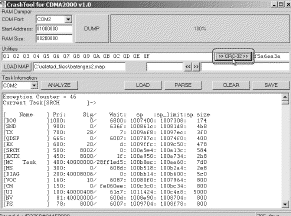
\includegraphics[width=.7\columnwidth]{featureful}
\caption{Internal tool for parsing the content in RAM.}
\label{fig:featureful}
\end{figure}

The above phenomenons were also observed in the early days of user
interface designs. Many new technologies---such as window, icon, menu,
and pointing device---had grasped the attentions of the software
developers. They were very eager to try out these new technologies and
often falsely believed that the implementation of these new
technologies were the goal of successful software.

This is indicated by \citet{inmates:cooper} that although software
developers work hard to make their software easy to use, their frame
of reference is themselves and as a result they make it easy for other
software developers, instead of typical end-users. He explains that
since having too much influence over the design of the human interface
and the lack of skills in this area, software developers do a poor job
of it.

\subsection{Usability and Interface Transparency}
% TODO: talk about user-centered design and usability
This situation will last until the software developers are introduced
to the concept of usability. Dated back since the 1980s, this concept
was introduced by the published studies and analysis papers from a
dedicated group of mostly psychologists and human factors researchers
\citep{human:rubinstein, friendly:simpson, human:shneiderman,
  human:brown, software:dumas}. The philosophy behind this is that
every stage of the development process---requirements, design,
implementation, verification, and maintenance---are given great
attention to the needs and limitations of the users.

In this user-oriented development, contrast to the previous
technology-oriented or feature-oriented development, software
developers work with experts from various specific fields---and most
importantly, also collaborate closely with the actual users---to bring
efficient, easy-to-learn, easy-to-memorize, and non-disruptive product
to the user. They form psychology and physiology models of the user to
anticipate their needs and limitations. And from that model, the
software developers could build products that perfectly fit the users
and not get in the way. Where the users can focus their attention on
the tasks at hand as if the user interfaces do not exist or seem
transparent \citep{computer:weiser}.

% Bring up transparency, disrupt
This interface transparency is an indication of good user interface
design. From their research, \citet{transparency:holtzblatt} show that
elements of an application design can disrupt users' work. They
observed that only when the users are not disrupted by the computer
system will they remain in the flow of their work and experience
interface transparency. It is also one of the ultimate goals for
usability studies and is considered the ideal relationship between
user and tool with the tool seeming to disappear by
\citet{transparency:rutkoski}.

\subsection{Danger of Transparency}
% danger of transparency
However, the idea of striving for interface transparency is at the
same time being challenged by others. \citet{windows:bolter} talked
about the myth of transparency: \textit{The danger of transparency is
  that the interface will mask the operation of the system exactly
  when the user needs to see and understand what the system is
  doing}. One reason for this danger comes from the fact that
designers and the users each have their own conceptual models or
mental images of the product. Ideally, these two models should be
identical for the users to understand and use the product
properly. Unfortunately, this might not always be the case. So the
users often have to form their own model exclusively from the
observation of the product, whether from the exterior guise, the
feedback provided, the responses from blogger, documentations, etc
\citet{design:norman}. But if the product was invisible or transparent
to the users, how could it act as a medium to help the users to
understand itself? Interface transparency eliminates the communicative
aspect of the user interfaces, along with others such as the engaging
aspect.

% other direction: user experience
% difficulty of user experience
The community of human-computer interaction quickly embraced the idea
that solely pursuing for interface transparency and performance is not
enough, and a richer model is required to encapsulate the other
perspectives of the user interaction. These all fall under the
umbrella term of user experience, which may include: addressing the
human needs beyond the instrumental; stressing affective and emotional
aspects of the interaction; and dealing with the nature of experience
\citep{ux:hassenzahl}. Many models have been proposed, however the
universal definition for user experience is still not well understood
nor fully clarified. There are several reasons why this is so,
according to \citet{ux:law} for example:
\begin{enumerate}
  \item User experience is associated with a wide range of vague and
    dynamic concepts, including emotional, affective, experiential,
    hedonic, and aesthetic variables. Whether or not to include each
    of these variables is greatly dependent on the interests and
    background of the proposing author.
  \item The unit for measuring user experience is
    \textit{malleable}. Unlike usability where only a single aspect of
    interaction between the user and the product is assessed with well
    defined criteria, it could be extended to include multiple users,
    environment while the product is being used, and more.
\end{enumerate}

\subsection{Definitions}
Some definitions of user experience are given here to illustrate its
diversity.
\begin{description*}
  \item[\citet{experience:alben}] \hfill \\
    All the aspects of how people use an interactive product: the way
    it feels in their hands, how well they understand how it works,
    how they feel about it while they're using it, how well it serves
    their purposes, and how well it fits into the entire context in
    which they are using it.

  \item[\citet{experience:nielsen}] \hfill \\
    All aspects of the end-user's interaction with the company, its
    services, and its product.

  \item[\citet{ux:hassenzahl}] \hfill \\
    A consequence of a user's internal state (predispositions,
    expectations, needs, motivation, mood, etc.), the characteristics
    of the designed system (e.g. complexity, purpose, usability,
    functionality, etc.) and the context (or the environment) within
    which the interaction occurs (e.g. organizational/social setting,
    meaningfulness of the activity, voluntariness of use, etc.)
\end{description*}


\section{Patterns Of User Experience}
\label{sec:pux}

Patterns of user experience, as described by \citet{pux:blackwell},
are a language for describing user experiences with structured
information. From the previous practices of and knowledge gained by
implementing software patterns, patterns of user experiences provide
familiar feelings to software developers. They are perhaps what the
software developers really need to improve the user experience of the
typical end-users, instead of the currently yet clarified definitions
and statements of user experience, and are also the one crucial factor
for this to succeed.

Interestingly, the traditional software patterns can also be
considered as patterns of user experience. But they are referring to
user experience for the \textit{software developers}, i.e.\ software
developers will have better experience with the source code if they
choose to implement the appropriate software patterns into their
design. For example, following a well known software pattern can
increase the maintainability of the source code among the
collaborating software developers.

However this intention for software patterns differs from the original
intention traced back since architecture and urban planning
\citep{timeless:alexander}. The original intention was to improve
comfort and quality of life for the people living inside. But due to
an early, albeit still existing, common misconception among software
developers, the intention of patterns turned in the wrong direction
when introduced to the software development domain. They often focus
too much attention on engineering the user interface and emphasizing
the technical details that, instead as supporting tools, these user
interface and technical details become the final product for the users
\citep{pux:blackwell}. That is why software patterns are applicable
toward themselves.

Nevertheless, the patterns of user experience we are focusing here is
the user experience for the \textit{users}, the actual users who will
be using the software. By implementing these patterns of user
experience into the design, the users can gain better user experience
with the product. Table~\ref{tab:shield} gives a simple example on
patterns of user experience for error management
\citep{patterns:welie}.

\subsection{Examples}
However the user experience we are mentioning here is the user
experience for the \textit{users}, the actual users who will be using
the software. By implementing these patterns of user experience into
the design, the users can gain better user experience with the
product. Table~\ref{tab:shield} gives a simple example on patterns of
user experience for error management \citep{patterns:welie}.

\begin{table}[!t]
  \caption{Pattern of user experience `The Shield'.}
  \label{tab:shield}
  \begin{center}
    \begin{tabular}{| p{0.2\columnwidth} || p{0.7\columnwidth} |}
      \hline
      Name & The Shield. \\ \hline

      Problem & The user may accidentally select a function that has
      irreversible (side) effects. \\ \hline

      Usability Principle & Error management. \\ \hline

      Context & The user needs to be protected against unintended or
      accidental actions that have irreversible (side) effects. The
      (side) effects may lead to unsafe or highly undesired
      situations. For example the unintended deletion or overwriting
      of files. Do not use for actions that are reversible. \\ \hline

      Forces & The user is striving for speed while trying to avoid
      mistakes. \\ \hline

      Solutions & Protect the user by inserting a shield. \\ \hline

      Usability Impact & Increased safety, less errors and higher
      satisfaction. However, it requires extra user action which leads
      to lower performance time. \\ \hline

      Rationale & The extra layer causes the user to require 2
      repetitive mistakes instead of 1. The safe default decreases the
      chances for a second mistake. \\ \hline

      Known uses & Microsoft Explorer, Apple Finder. \\ \hline
    \end{tabular}
  \end{center}
\end{table}

\subsection{For Interface Transparency}
% Talk about various other non interface transparency.
% Talk about Linux and Windows as example for transparency.

% * Different meanings of interface transparency.
% * Brief mentioning of interface transparency in the history of
%   human-computer interaction.

Though there are quite a few existing publications discussing patterns
of user experience in various aspects of human-computer interaction
(refer to section \ref{sec:related}), we will focus our attention on
investigating the patterns of user experience for interface
transparency.

Interface transparency often have different meanings when presented to
diverse set of audiences. For expert system, interface transparency is
important for gaining trust to the users [FIXME].

Similarly, for Unix power users following the Unix philosophy,
interface transparency might suggest that the software is capable of
churning out excessive amount of messages when error occurred. These
power users are able to interpret the messages and partially `replay'
the flow of control\footnote{Refers to the order in which the
  individual statements or instructions of a program are executed or
  evaluated.}  for the software. The software at fault is not a
completely opaque black box to them with the help of the
messages. They can sort of see through the software and figure out the
problem hiding underneath \citep{unix:raymond}.

On the other hand, typical end-users do not usually consider excessive
messages as interface transparency. A common action when typical
end-users encounter unexpected information: they try to get rid of it
as soon as possible \citep{oldnew:chen}. To them, the information are
regarded as either gibberish or elaborated way of describing something
dangerous. This is because the information is unforeseen and cannot
fit into the conceptual model which they had previously formed for the
software. Hence, instead of being treated as interface transparency,
the excessive messages are more like an unknown dark spot occluding
the flow of experience\footnote{Refers to the mental state of
  operation in which a person is fully immersed in a feeling of full
  involvement in the process of an activity.}.


% Form pattern and guidelines for software developer, with respect to
% interface transparency.
[Elaborated paragraphs explaining interface transparency as my second
  research interest.]

Added to this, the emergence of the user experience is an attempt to
inform design and evaluation has been widespread in HCI. Such that,
researchers are proposing user experience encapsulating the idea of
interface transparency.

Hence, the relationship between transparency and user
experience will also be examined.


\section{Planned Experiments}
\label{sec:experiment}
[FIXME]

\subsection{Research Goal}
[Elaborated paragraphs combining patterns of user experience and
  interface transparency as my research goal.]

% problem I am trying to solve
With all this being said, this article is not another attempt to
develop a common view on user experience. Numerous literature,
conferences, and workshops have already attempted to address this
topic, such as \citet{early:forlizzi}, \citet{emotional:norman},
\citet{action:dourish}, \citet{ux:hassenzahl},
\citet{experience:desmet}, and \citet{ux:law}.

For sake of completeness, some view points on user experience will
still be discussed in the following section. However, the main
research goal for this article is to further explore interface
transparency within the field of user experience. Interface
transparency is still a crucial factor in this field, even though user
experience has been the prominent subject in recent years. In his
article, \citet{future:memmel} suggests that usability engineering and
interaction design will be the more concrete premises and disciplines
below the umbrella term of user experience. This argument is similar
to the one from \citet{windows:bolter} that transparency is only half
the story---each digital design should move back and forth between
being transparent and being reflective.

Transparent and reflective, two contrasting albeit interesting point
of views prompted people to think about whether they have been too
obsessed with achieving interface transparency, the benefits and
limitations of interface transparency, measuring interface
transparency. Added to this, the emergence of the user experience is
an attempt to inform design and evaluation has been widespread in
HCI. Such that, researchers are proposing user experience
encapsulating the idea of transparency. Hence, the relationship
between transparency and user experience will also be examined.

% Talk about the experiment.
\subsection{Experiment}
[FIXME]

A new human interface device and application will be developed to
investigate interface transparency within user experience. This new
device will provide similar functionality to the multi-touch touchpad
that comes with recent laptops. However, the device will enable the
users to perform the usual tasks of multi-touch touchpad on any
surface, as if the physical touchpad is underneath their hand. The
development of this new device is actually based upon our previous
study \citep{lmnt:huang}, where the first-generation prototype was
built and some preliminary studies were conducted. Much of the
feedback from the first-generation prototype are taken into
consideration when designing the new device for this study.

% Application based on Baba Painter.
An application will be developed to accompany the new human interface
device. This application will too be an extension to our other
previous study, an interactive painting and collaboration reviewing
system \citep{baba:abeyrathne}. However, since the instrument will be
replaced by the new device developed in this study, the scenario and
the users will be adjusted accordingly. We planed to target the
application to kids. The application will allow small children to
scribble intuitively on any surface and be creative wherever they are,
whether on the dining table of a restaurant or on the wall in the
bedroom, while without causing any mess or damage.

% User, product, context


\section{Conclusion}
\label{sec:conclusion}
[FIXME]


\bibliographystyle{apalike}
\bibliography{final}


\end{document}
